\documentclass{article}

\usepackage{fullpage}
\usepackage{titlesec}
\usepackage{parskip}
\usepackage{graphicx}
\usepackage{bold-extra}
\usepackage{caption}
\usepackage{subcaption}

%\titleformat{\section}{\normalsize\bf}{\thesection \hspace{5pt}}{0em}{}
%\titleformat{\subsection}{\normalsize\bf}{\thesubsection \hspace{5pt}}{0em}{}
\title{Distributed Multi-Heuristic A* (HAMSTAR)}
\author{Noam Brown, Aram Ebtekar, Yuzuko Nakamura
\\15-712 Fall 2014 Final Project Report}

\begin{document}
\maketitle

\begin{abstract}
A* is a popular graph search algorithm used in many artificial intelligence applications. The original A* algorithm uses a single heuristic to prioritize exploration through a graph, but a variation on the algorithm known as shared multi-heuristic A* (SMHA*) makes use of multiple heuristics to more quickly arrive at near-optimal solutions. For this project, we implemented a distributed version of SMHA*, separating each heuristic into a separate process. We compare the results of our distributed implementation to the original SMHA* algorithm. In particular, we provide evidence that in domains where state expansions are expensive, our distributed approach may outperform SMHA*.
\end{abstract}

\section{Introduction}

Weighted A* is a simple, heuristic-based search algorithm used in artificial intelligence applications such as robotics and games. A heuristic function estimates the remaining distance from any state to the goal. Whereas a breadth-first method such as Dijkstra's algorithm will expand exponentially many states relative to the goal distance, wA* will focus toward the goal when guided by a good heuristic. If the heuristic is \textbf{admissible}, meaning it never overestimates the true distance, then the solution is guaranteed to be optimal to within the weight factor. If it meets a stronger condition called \textbf{monotonicity}, then no state needs to be expanded more than once.

Finding good efficiently computable heuristic functions is difficult and, moreover, finding an admissible heuristic function that is reasonably accurate over the entirety of the search space is often not practical. Multi-heuristic A* (MHA*) \cite{Aine14} is an alteration of the A* algorithm that allows multiple arbitrary heuristics to guide the search; to retain the optimality bound, it is only necessary to use one monotone heuristic, called an ``anchor". Where the shortcomings of each individual heuristic may result in local optima which trap the search, the ability to change heuristics can provide an escape.

In their work, Aine et al. propose MHA* in two flavors: Independent Multi-Heuristic A* (IMHA*), where path cost and shortest path information are tracked separately for each heuristic, and Shared Multi-Heuristic A* (SMHA*), where shared knowledge of path cost and shortest path information are shared and updated by all heuristics. IMHA* would be almost trivial to parallelize, as it requires minimal communication between the searches run by different heuristics. SMHA* uses a very large amount of frequently updated shared memory, presenting major challenges for parallel settings, let alone distributed systems settings.

Nonetheless, as SMHA* is the more effective of the two (enabling more co-operation and less redundancy between heuristics), we decided for our project to implement a distributed version of SMHA*.

\section{Relevant Work}

Our work is directly based on Aine et al.'s original multi-heuristic A* search \cite{Aine14} mentioned above. There exists past work on the paralellization of A*; in particular, Phillips et al. \cite{phillips2014pa} were able to achieve parallelization while retaining wA*'s guarantee of suboptimality without reexpansions. This method of parallelization makes inferences on when it is safe to expand multiple states in parallel, by resolving dependencies between potential optimal paths. Their speed gains are dependent on the expansion operation being expensive enough to dominate the cost of computing these dependency checks, which may not be the case for all problems. By contrast, our method parallelizes the search process by simultaneously expanding states chosen by different heuristics, instead of multiple states chosen by a single heuristic. We allow each state to be expanded by each heuristic at most once and, furthermore, no state will be expanded by a non-anchor heuristic which has received a message from another heuristic after the latter has expanded the same state. In other words, aside from communication latency, no state will be expanded more than twice.

\section{System Description}

\begin{figure}[h]
\centering 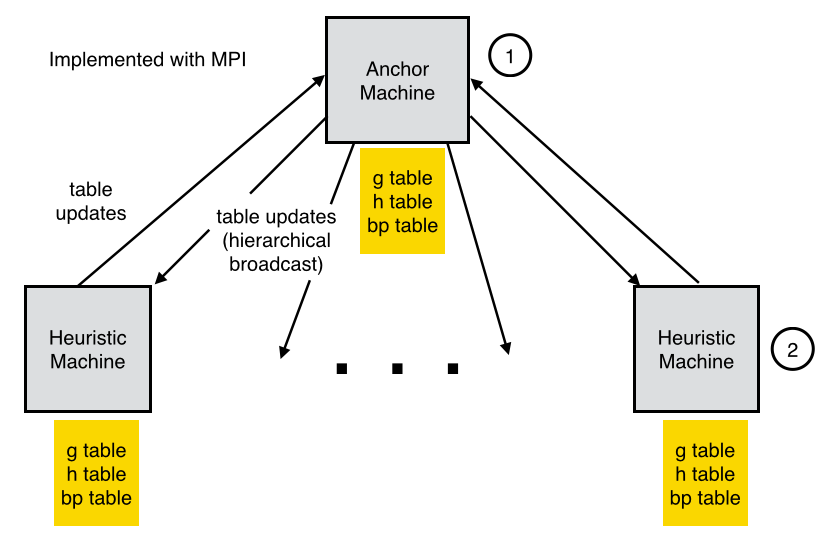
\includegraphics[width=5.0in]{system-diagram}
\caption{A diagram of our system. One machine starts up the others and runs the monotone anchor search. The other machines run their individual heuristics. Communication is done using MPI. 
\textcircled{1}\textbf{Anchor:} Starts heuristic machines; performs state expansions using anchor heuristic; receives, resolves, and broadcasts table updates; checks for termination conditions. \textcircled{2}\textbf{Heuristic:} Expands a likely state (chosen using heuristic); updates path cost to its successors; communicates updates to anchor; checks for termination conditions}
\label{fig:sysdiag}
\end{figure}

An overview of our system is in Figure \ref{fig:sysdiag}. The main (anchor) machine starts up other heuristic machines. Each machine runs its own heuristic, with the anchor machine's being the monotone heuristic. Each of the non-anchor heuristic machines periodically sends updates of the data structures (tables containing shortest path information found so far) to the anchor machine, which compares the data it receives and sends out table updates of the best paths known so far to all other states.



\begin{figure}[h]
\centering
\begin{subfigure}{3in}
  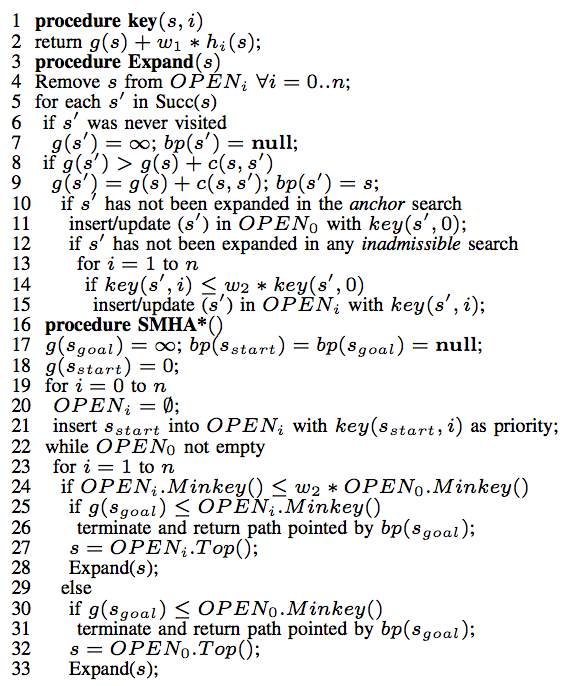
\includegraphics[width=3in]{pseudocode}
  \caption{Pseudocode}
  \label{fig1}
\end{subfigure}
\begin{subfigure}{2in}
  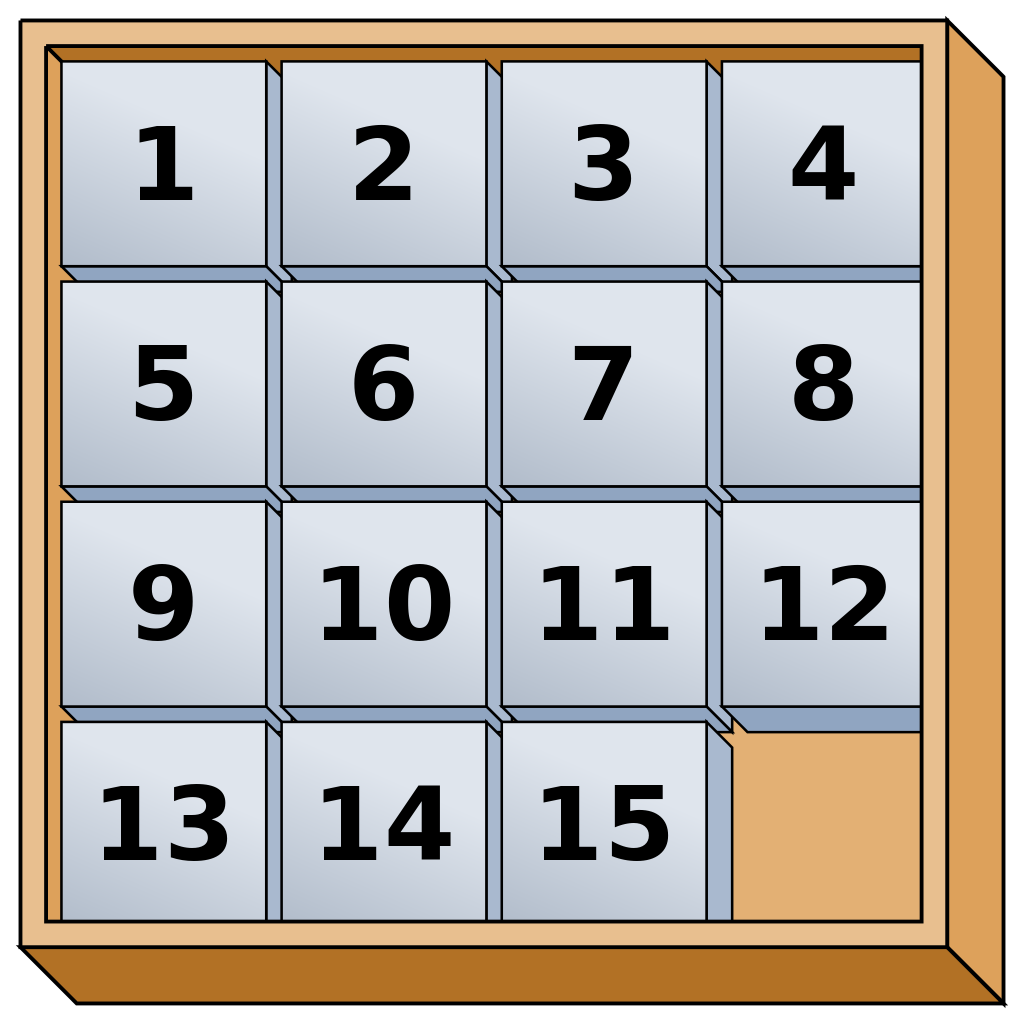
\includegraphics[width=2in]{graphs/puzzle}
  \caption{15-puzzle goal configuration}
  \label{fig2}
\end{subfigure}
\caption{Pseudocode from Aine et al., detailing the original sequential version of the algorithm we parallelized, alongside the sliding tile puzzle which we use it to solve.}
\label{fig:pseudocode}
\end{figure}


Our algorithm is based off of the sequential, round-robin SMHA* code presented in \cite{Aine14} (Figure \ref{fig:pseudocode}). Our parallelized code was written in C++ with inter-process communication accomplished using MPI. The work was distributed over one or more of the 16-core machines in the Apt cluster. We associate one heuristic with each process that we run. In the following sections, we may use the terms machine and process interchangeably, even though we also tried running multiple heuristics (one per process) on one multi-core computer.

\subsection{Design Decisions}

\subsubsection*{Interprocess communication with MPI}

We investigated other frameworks designed for iterative algorithms on a stable dataset such as Spark and GraphLab. However, most of these frameworks were designed for chunking up a large dataset and assigning pieces to workers. Our application's needs differed from this model in that the dataset being operated on (the graph being explored) was shared by all workers, and the workers themselves were performing differing operations on subsets of the same data.

We chose MPI, despite its complexity and low level of abstraction, because our algorithm requires extremely fast and efficient communication between the anchor and the child machines. Moreover, since the entire state must be replicated across all machines, the necessary communication was relatively straightforward. Finally, we found that detailed documentation on MPI, explaining the low-level workings of each command, was much more readily accessible than comparable documentation on Spark or GraphLab, which seemed more focused on abstracting the details of the system away from the programmer. Given our emphasis on speed, MPI seemed like an appropriate choice. We ultimately used the OpenMPI implementation of the MPI standard.

\subsubsection*{Synchronous broadcast vs. one-on-one communication}

We considered two communication models for our algorithm. The first, which we call the one-on-one model, has the anchor periodically send all children a table of states. The table contains information for new states that were either received or calculated by the anchor since its most recent communication with this child. Each child frequently checks for incoming messages using the \emph{MPI\_Iprobe} command: if a message is detected, the child receives the incoming data using \emph{MPI\_Recv} and responds with its own table of states. The anchor sends messages to each child one at a time, moving on to the next child when a response is received. Once the data has been sent to all children, the anchor will run its own expansion iterations until a time when the next cycle should begin.

The second communication model involves a periodic broadcast using the \emph{MPI\_Bcast} command. After a pre-determined number of iterations, all child machines send their new or updated states to the anchor using \emph{MPI\_Gather}. The anchor sifts through these responses, and keeps only the best $g$-value for each state. Every state that has had a new best $g$-value found is then broadcast to all the child machines.

The one-on-one communication model has the benefit that it does not require all machines to cease work while communication happens; only the anchor and a single child machine need to participate in the communication. The downside is that the anchor must then do $O(N)$ communications, where $N$ is the number of children, and the time it takes to propogate the new state tables across the entire system is also $O(N)$. Broadcasts, on the other hand, require a simultaneous call from all machines. This generally requires more overhead, because it is unlikely that all machines will call the command at precisely the same time. However, once called, the Broadcast command allows the anchor to only send the data to a few machines in the network. These machines, in turn, forward the data to other machines, and so on. Thus, the anchor does not spend significantly more time communicating than other machines in the system, and the new state table is propagated in $O(\log(N))$ time.

We ultimately chose the broadcast model for our implementation due to the more balanced workload on the anchor. In fact, for the case of the sliding tile puzzle, the one-on-one communication model was not a viable option; it would take longer for the anchor to process incoming states and send them out than it would for child machines to expand new states.

\subsubsection*{Update collation performed at anchor machine}

SMHA* needs to share the values of $g$ (distance estimates) and $bp$ (back-pointers) for every state. As sharing memory is infeasible in our distributed implementation, processes periodically broadcast their $g$ and $bp$ values to update one another. This can result in conflicting data for a particular state, which is resolved by taking the data which gives the lowest $g$ value for that state, as it contains the best estimate found so far. During conflict resolution, we also take the inclusive OR of the flags specifying whether the state has ever been expanded by the anchor, or by any machine at all. This prevents unnecessary reexpansions.

Each message only needs to contain the portion of the graph which has been updated by the sending machine since its most recent network communication. Nonetheless, if every machine broadcasts its updates directly to all other machines, the network would flood with messages and much conflict-resolution work would be duplicated. Therefore, we instead have every machine send its table updates exclusively to the anchor machine. The anchor alone takes the burden of resolving all conflicts between duplicate states, and then periodically broadcasts the merged collection of updates to all machines.

The disadvantage is that we rely heavily on the anchor machine functioning reliably. This is a small price to pay, given that the anchor is already necessary for updating the optimality bound. To avoid unduly burdening the anchor, every machine is able to compute the anchor heuristic and includes its value in the state updates it sends to the anchor machine. Finally, the anchor machine's broadcasts also include its latest lower bound on the optimal solution cost, enabling child machines to deduce when they are below the $w_1w_2$ optimality factor.

\subsubsection*{Back-pointer optimization}

$bp(s)$ represents the parent of $s$ along the optimal path found so far from the start to $s$. As a single pointer cannot be shared across a distributed replicated data structure, our first implementation used a full state representation (5x5 puzzle configuration) in place of $bp(s)$, nearly doubling the length of network messages. However, notice that $bp(s)$ is not needed to perform the search $g$-value computations; it is only needed to reconstruct the solution path once the search terminates.

Therefore, it suffices to use pointers referring to the machine's local entry for that state. These pointers need not be communicated until the search terminates. At that point, the path can be obtained by walking backwards from the goal. At each step, we move from the current state $s$ to the neighbor $s'$ which minimizes $g(s') + c(s',s)$ among the possible parents $s'=bp(s)$ pooled from all machines. Although we still end up sending full state representations, these are only for the parents of states along the path, rendering the overhead negligible.

\section{Experimental Setup}

We tested our algorithm on the 24-puzzle, a 5x5 grid of sliding blocks which must be rearranged to achieve a standard goal configuration, somewhat akin to solving a Rubix cube. Uniformly at random, we generated 10 starting configurations among the over $3\times 10^{23}$ states of the puzzle. The data we collected were (1) running time, (2) total number of states in the problem graph that were expanded across all processes during the search, and (3) the length in steps of the best solution at termination. For each of these, we discard the top and bottom value. Our plots show the min, mean and max of the 8 remaining values. Our main evaluation criterion is the time to complete the search with the required suboptimality guarantee, which we fix to $w_1 w_2 = 4$.

The anchor heuristic is $h(s) = MD(s) + LC(s)$ where $MD(s)$ is the sum of Manhattan distances of each non-blank tile to its destination, and $LC(s)$ is the linear conflicts heuristic which essentially adds 2 for each pair of horizontally or vertically aligned times which need to pass each other. This heuristic is admissible, in fact it's monotone. Additional heuristics are generated randomly from $MD$, $LC$, and the misplaced tiles heuristic $MT$ which simply counts the number of non-blank tiles which are not already at their destinations. We randomly generate a triple of coefficients, each between 1 and 5, to form a linear combination of these heuristics. We repeat this process as many times as we require non-anchor heuristics. These heuristics are not at all admissible, and their high values give the search a goal-directed focus as the anchor typically underestimates the true distance by a large margin.

SMHA* specifies two weight parameters. The first weight ($w_1$) gives the search a more depth-first goal-directed focus. The second weight ($w_2$) determines the margin by which a proposed solution's cost may exceed the anchor's minimum frontier key value, which is itself $w1$ times a lower bound on the optimum solution cost. Therefore, SMHA* guarantees that the solution found at termination is at most $w_1 w_2$ times the optimum value. This guarantee applies equally well in our distributed variant. For all experiments, we used $w_1 = w_2 = 2$. Every state expanded by the anchor has a $g$ value which is optimal to within a factor of $w_1$.

\section{Results}

Figure \ref{fig1} plots runtime as we increase the number of processes (or heuristics, in the case of SMHA*). As shown, performance increases significantly at first, but then drops off as the number of processes increases. When running on a single machine, our distributed algorithm performs comparably to SMHA* for 4 or fewer cores, but decreases in performance as more processes are added.

There are a number of likely explanations for this. First, the initial performance increase is largely a result of adding a heuristic with a greedier bias, typically finding a slightly less optimal path more quickly. Indeed, figure \ref{fig2} shows that the solution length increases considerably after adding just one non-anchor process. However, it is worth noting that our criterion is specifically to find a path whose cost is within the specified multiple (in our case, 4) of the optimum. Crucially, the combination of monotone and inadmissible search is able to guarantee the near-optimality of the solution; thus, the slightly longer path is viewed as an equally valid solution. The additional heuristics provide more variety in the search, making it more likely for at least one of them (or some combination) to succeed in finding a good path. The drop in performance as more processes are added appears to be due to the increased communication cost of using a broadcast communication system. All processes must pause for this, and some might be slow in calling the broadcast command. Moreover, as more processes are added, the anchor receives more states that it must sift through, and the following message that it broadcasts increases in size as well. Thus, it appears that after a sufficiently diverse group of heuristics is added, the added communication cost of additional heuristics outweighs the benefits. These communication costs are analyzed in more detail later in this section and are displayed in figure \ref{fig5}.

Figure \ref{fig3} shows performance as we vary the number of iterations between communications. For reference, 100 iterations in our experiments takes roughly 1-5 milliseconds. As one would expect, very frequent communication eventually causes the communication overhead to grow too large and hurts performance.  On the other hand, as communication becomes extremely infrequent, the lack of shared information also hurts performance considerably. The optimal communication interval therefore depends heavily on the nature of the problem; in our case, it appears to be around 6,400 iterations.

As discussed earlier, our algorithm does not appear to outperform SMHA* in the sliding tile puzzle domain. The most likely explanation for this is that, because the successor states and heuristics we used for the puzzle can be calculated extremely efficiently, there are a huge number of expansions per unit time. Each expanded state must be communicated to the anchor, which involves a considerable amount of work. It is likely that the amount of work in sending the states to the anchor, having the anchor process these states, broadcasting the best of those states to the other children, and having those children process the states, altogether takes about as much work as expanding the state alone. Indeed, figure \ref{fig5} shows that as the number of processes increases, communication quickly becomes a huge fraction of the total time spent. This increased communication cost ultimately outweighs the benefits of additional processes.

Nevertheless, figure \ref{fig4} displays what the results might look like in a problem where the heuristic takes longer to calculate. Specifically, we artificially slow the heuristic calculation by a factor of 10. The result is that fewer states are expanded per second, and thus the cost of communicating a state is much lower relative to the cost of expanding it. In this case, our distributed algorithm can leverage the benefit of additional cores to outperform SMHA* if we use the one-on-one communication method described earlier in this report. Thus, a distributed approach may prove helpful in domains such as manipulator arm planning, in which expansions are slowed by the collision checking and numerical integration needed to compute successor states and heuristics.


\begin{figure}
\centering
\begin{subfigure}{3.2in}
  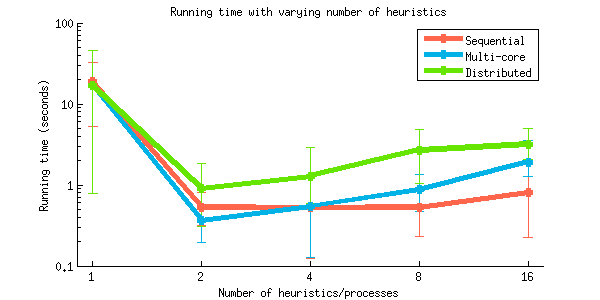
\includegraphics[width=3.2in]{graphs/figure1}
  \caption{Running time}
  \label{fig1}
\end{subfigure}
\begin{subfigure}{3.2in}
  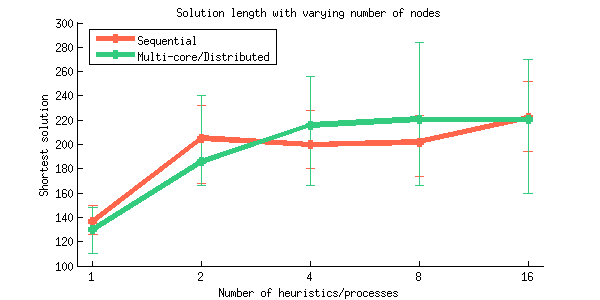
\includegraphics[width=3.2in]{graphs/figure2}
  \caption{Solution length}
  \label{fig2}
\end{subfigure}
\caption{Comparison with Runtime performance and solution quality as the number of different heuristics (cores) on a single machine increases. Communication occurs every 5,000 iterations.}
\label{fig:singthread}
\end{figure}

\begin{figure}
\centering
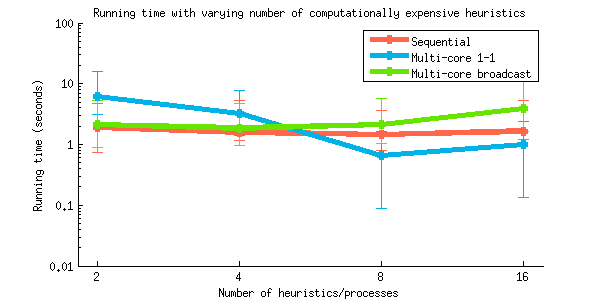
\includegraphics[width=3.2in]{graphs/figure3}
\caption{Runtime performance as communication frequency is varied. Experiment was done on 2 machines, with 2 processes on each machine.}
\label{fig3}
\end{figure}

\begin{figure}
\centering
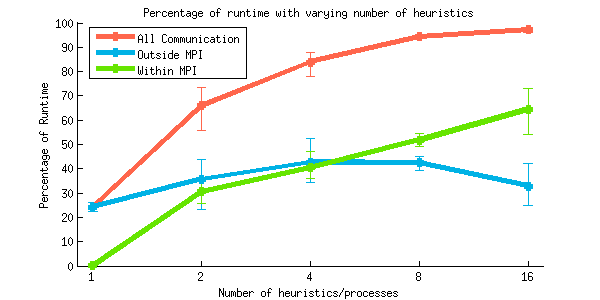
\includegraphics[width=3.2in]{graphs/figure5}
\caption{Cost of communication as the number of processes increases. Each process is on a different machine. Communication occurs every 5,000 iterations. Within MPI refers to only MPI commands. Outside MPI refers to other communication, such as serializing and reading states.}
\label{fig5}
\end{figure}

\begin{figure}
\centering
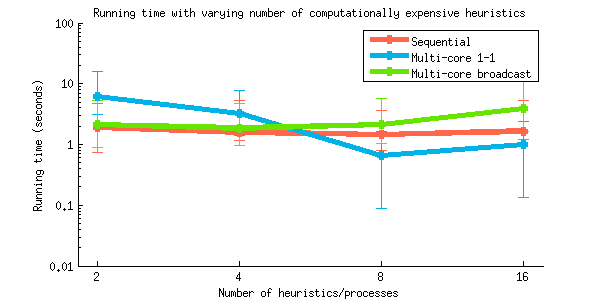
\includegraphics[width=3.2in]{graphs/figure4}
\caption{Performance of distribution on heuristics that are 10x slower. Since each iteration is slower, we communicate every 1,000 iterations instead of every 5,000 for this experiment.}
\label{fig4}
\end{figure}


\section{Conclusions}


In this report, we outlined the details of a distributed version of the SMHA* algorithm. We detailed the implementation of the algorithm, and presented experimental results comparing its performance while varying a number of parameters. We also compared its performance to the original SMHA* algorithm.

In the specific domain we tested on (the sliding tile puzzle), our distributed algorithm did not outperform the original SHMA*. The culprit appears to be the excessive communication cost relative to the cost of expanding a state. We were partially able to mitigate this by using the broadcast model of communication, and by reducing the footprint of a communicated state by not recovering the backpointer until the end and by offloading the calculation of the anchor heuristic onto the child machines. Nevertheless, it appears more optimizations would be required in order to gain a significant benefit over vanilla SMHA*. One possibility is the use of asynchronous communication. Both of our communication models required the sender and receiver to be ready to communicate simultaneously. If one was ready before the other, then that machine would be blocked until the counterpart responded. Using asynchronous communication would eliminate the requirement that all machines cease work until all are ready which, due to the likelihood of slow outlier machines, becomes a more significant problem as the machine count increases. This would also make the algorithm more robust to failure, since the algorithm could proceed even if some machines become unresponsive. The latest version of MPI (MPI 3.0) appears to include an asynchronous broadcast option that would accomplish something similar to this.

Although our distributed algorithm did not outperform SHMA* on the sliding tile puzzle, we have provided evidence that our algorithm could outperform SMHA* in domains where heuristics are difficult to calculate, or in general where state expansion is expensive.


\bibliographystyle{ieeetr}
\bibliography{sources}

\begin{figure}[b]
\centering

\includegraphics[width=0.49in]{graphs/hamstar}
\end{figure}



\end{document}